\anothertitle{Introduction and Terminology}{}

\begin{frame}
  \Frametitle{Introduction}

  \begin{itemize}
    \item Introduction and Problem Description
    \item Methodology and Process
    \item Results and Discussion  
    \item Conclusion and Future Work
    \item Questions
  \end{itemize}
  
\end{frame}

\begin{frame}
  \Frametitle{Goal}

  \begin{columns}
    \column{0.4\textwidth}
      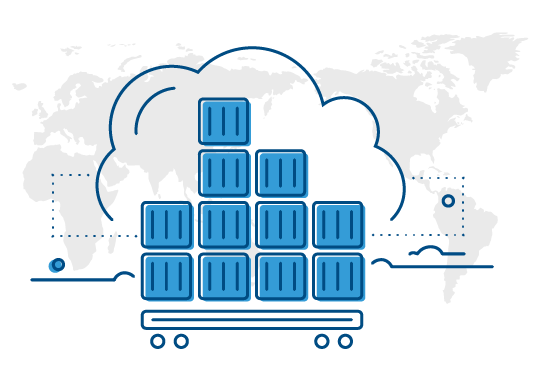
\includegraphics[keepaspectratio,width=\textwidth,height=\textheight]{cloudContainer}  
  
    \column{0.6\textwidth}
      \bullettext{This project aimed to compare \emph{Cloud Container Orchestration} platforms in respect to}:
      \begin{itemize}
            \item \bullettext{ease of adoption and configuration}
            \item \bullettext{deployment process}
            \item \bullettext{restrictions and limitations}
            \item \bullettext{performance}
            \item \bullettext{cost impacts}
            \item \bullettext{reliability and resilience}
      \end{itemize}

    \end{columns}
  
\end{frame}

\begin{frame}
  \Frametitle{Delimitations}
  
  \vspace{15pt}
  \bullettext{This project was restricted to investigation and experimentation pertaining to:}
  \begin{itemize}
    \item \bullettext{container-based workloads}
    \item \bullettext{the Amazon Web Services Cloud provider}
  \end{itemize}
  \begin{center}
    
\includegraphics[scale=0.25,keepaspectratio]{aws_logo} 
  \end{center} 

\end{frame}

\begin{frame}
  \Frametitle{Basic Terminology}

  \begin{itemize}
    \item \bullettext{\textbf{Cloud Computing} - computational resources made available to end-users on-demand over the internet, 
      usually charged per resource consumed.}
    \item \bullettext{\textbf{Containerization} - Operating System Virtualization - 
      packaging an application and its dependencies with a light-weight OS, 
      which is run inside a host system using instructions native to the core CPU} 
    \item \bullettext{\textbf{Serverless Computing} - computing paradigm where cloud providers abstract away the concept of servers,
      instead creating and allocating resources automatically on-demand}
    \item \bullettext{\textbf{Infrastructure as Code (IaC)} - using 'code' manifests to define, configure, and maintain infrastructure resources}
  \end{itemize}
  
\end{frame}